\section{Evaluation and Test Suites} \label{sresults}

For models using aggregated data dependences, Embla~2 must be run twice---first
to collect all observed dependences, and then to calculate a parallelism figure
given those dependences. When run on an x86 desktop, the first run causes an
average of 1500x slowdown of the profiled program, while the second run causes
an average of 700x slowdown.  Most of the slowdown is attributed to garbage
collection.  Valgrind itself, on which Embla~2 is based, causes a slowdown of
8x on average.

We demonstrate the usefulness of Embla~2 using example Cilk programs packaged with the 5.4.6 release of Cilk,
as described in Table~\ref{cilk-ex}\footnote{We
have omitted programs that use the \texttt{inlet}, \texttt{abort} and \texttt{SYNCHED} keywords,
as their translation into ordinary C is not straightforward.}.
As examples packaged with a parallel programming environment,
these are programs known to have lots of task-level parallelism.
Furthermore, the nature of Cilk means that these programs can be translated into semantically equivalent programs in ordinary C (known as \emph{serial elisions}) simply by stripping the Cilk keywords\footnote{Namely,
\texttt{cilk}, \texttt{spawn} and \texttt{sync}.}.
We thus have a set of C programs and their manually-parallelized counterparts to compare with the parallelism discovered by Embla~2.

\begin{table}[t]
\centering
\scriptsize
\begin{tabular}{ | l | l | l | }
\hline
Program & Description & Parameters \\
\hline
\textsf{cholesky} & Matrix decomposition & \texttt{size=256}, \texttt{nonzeros=1000} \\
\textsf{cilksort} & Merge sort & \texttt{size=100000} \\
\textsf{fft} & Fourier transform & \texttt{size=512*512} \\
\textsf{fib} & Na\"ive Fibonacci calculation & \texttt{n=30} \\
\textsf{heat} & Differential equation solver & \texttt{nx=ny=512}, \texttt{nt=1} \\ 
\textsf{lu} & Matrix decomposition & \texttt{n=256} \\
\textsf{magic} & Magic squares search & \texttt{n=4} \\
\textsf{matmul} & Matrix multiplication & \texttt{n=128} \\
\textsf{plu} & Matrix decomposition & \texttt{n=128} \\
\textsf{strassen} & Matrix multiplication & \texttt{n=512} \\
\hline
\end{tabular}
\small
\label{cilk-ex}
\caption{Description and parameters for Cilk 5.4.6 examples used}
\end{table}

\subsection{Finding optimal task synchronization points} \label{sresults:cilk-spawns}
\begin{figure}[t]
  \begin{center}
  \scriptsize
  \input{cilksort.depgraph}
  \end{center}
  \caption{An extract from \textsf{cilksort} and its corresponding relevant dependences}
  \label{cilksort-depgraph}
\end{figure}

Programmers can use aggregated dependences discovered by Embla~2 to realize the parallelism discovered using a language like Cilk,
where function calls are spawned as tasks and later joined (or \emph{synchronized}),
by synchronizing on previously spawned tasks just before the first line dependent on them.
As an example, Figure~\ref{cilksort-depgraph} shows an extract from the \textsf{cilksort} program,
along with aggregated dependences discovered by Embla~2 on the program's serial elision.
By spawning function calls and synchronizing before the first line that depends on previously spawned tasks,
we arrive at the Cilk program with optimal parallelism, which in this case is the same as the original program.
However, the programmer should be aware that as with all dynamic analyses,
these dependences are based on running the program on sample inputs only and so the parallelization may not be safe for all possible inputs.
Nevertheless, previous work~\cite{embla:08} has shown a correlation between dependence coverage and code coverage.

\subsection{Amount of parallelism discovered} \label{sresults:cilk-limits}

Figure~\ref{cilk-run} compares (on a logarithmic scale) the amount of parallelism found by Cilk's timing infrastructure (averaged over 60 runs) to that found by Embla~2 on their serial elisions.
Our baseline model for this comparison uses aggregated data dependences, and considers only function-call-level parallelism without loop parallelization or spawn hoisting---the closest model we have to Cilk's.
The graph shows that Embla~2 is able to find all of the task-level parallelism in most of the original Cilk programs.
One notable exception is \textsf{magic},
and this is because the Cilk program uses an implicit \emph{inlet}\footnote{In Cilk an \emph{inlet} is a block of code that is executed atomically after a task completes. The potential thread contention for such an atomic block might explain the large variance in actual parallelism in the Cilk run.} at the statement \texttt{count += spawn execute(...);},
which is not a feature of our model.
Later we show how, by extending our model, Embla~2 also discovers the parallelism here.

For a few examples Embla~2 can discover more parallelism than explicitly specified in the original Cilk program.
We found several functions called synchronously that could have been spawned,
as well as C library function calls
that can be spawned with the addition of simple wrappers.

\begin{figure}[t]
 \begin{center}
  \begin{SubFloat}{\label{cilk-run}Parallelism of Cilk programs as calculated by Cilk and Embla}
   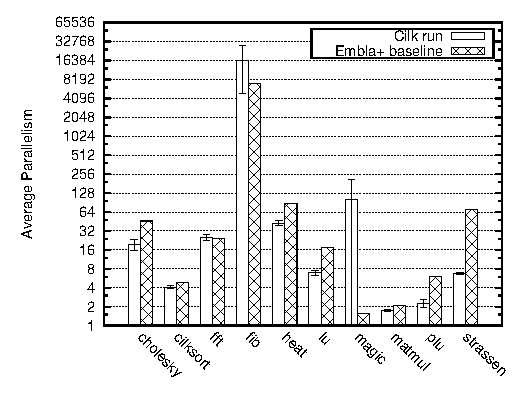
\includegraphics[width=2.0in]{cilk-run}
  \end{SubFloat}
% \end{center}
 \qquad
% \begin{center}
  \begin{SubFloat}{\label{cilk-gran-loop}Parallelism of Cilk programs using variant models}
   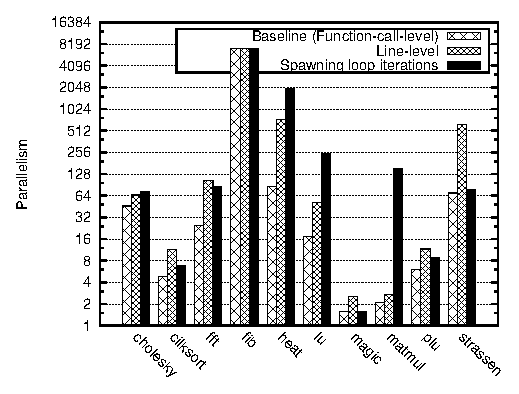
\includegraphics[width=2.0in]{cilk-gran-loop}
  \end{SubFloat}
 \end{center}
 \caption{Parallelism of Cilk programs (note logarithmic scale)}
\end{figure}

\subsection{Effects of optimizations} \label{sresults:cilk-opts}

We now look more closely at the variant optimization models to see whether they affect potential parallelism in these programs.

\paragraph{Exact data dependences}
In most programs in the Cilk test suite the difference between this model and the baseline is negligible.
This suggests that for such programs most of the potential parallelism is statically achievable---runtime techniques such as thread-level speculation (TLS) would give few performance benefits.
One exception is \textsf{lu}, which gives an almost-fourfold speed-up over the baseline.
This is because in one nested loop the dependence for a certain task on itself exists only between iterations of the outer loop but not of the inner loop.
With aggregated dependences this results in all instances of the task being serialized, while with exact dependences instances from the same iteration of the outer loop can still be parallelized.
While TLS would address this issue, a cheaper method is to parallelize the inner loop---part of the speed-up seen in the third columns of Figure~\ref{cilk-gran-loop} can be attributed to this task.

\paragraph{Line-level parallelism}

The amount of line-level parallelism in these programs is compared to the amount of function-call-level parallelism in Figure~\ref{cilk-gran-loop}.
We can see that for most of these programs the amount of line-level parallelism is around twice or more that of function-call-level parallelism.
This is mostly due to simple statements performing arithmetic operations inside a function call or loop that can run in parallel.
Each of these operations takes a small number of cycles, which means that it is not viable for each of these to be spawned.
As mentioned, some of this fine-grain (mostly instruction-level) parallelism is realized already in existing superscalar processors.
Nevertheless, operations may be grouped and extracted into tasks that are sufficiently large to see performance gains.

\paragraph{Loops}

Looking at the first and third columns of Figure~\ref{cilk-gran-loop}, which
compares the potential parallelism of Cilk programs without and with spawning loop iterations, we can see that the use of parallel for-loops benefits most of the programs considered here.
This is most remarkable in \textsf{matmul}, where there is a 64-fold gain in parallelism when for-loops are parallelized.
This confirms the view that the use of parallel for-loops is an excellent way to express task-level parallelism, in addition to function calls.
Furthermore, some parallel programming environments (e.g.\ Cilk++~\cite{leiserson09cilk}) optimize parallel for-loops by deriving loop induction variables by divide-and-conquer instead of linearly,
meaning that actual parallelism may be even higher than these figures.
Embla~2 not only finds the amount of loop-level parallelism in a program, but can be used to easily identify candidate loops for parallelization.
This can simply be done by searching through the dependences output by Embla~2 for dependences between iterations of the loop concerned.
If there are no such dependences, then the loop can be parallelized.

\paragraph{Reduction operations}

When dependences between reduction operations are discounted,
the parallelism of \textsf{magic} vastly increases from under 2 to 376.
This means that a parallel reduction mechanism, such as Cilk's implicit inlets, \emph{hyperobjects} in Cilk++ and similar operations in OpenMP,
is essential for the program's parallelism potential to be realized.

\paragraph{Spawn hoisting}

With these Cilk programs, we find that spawn hoisting has a negligible effect on the amount of potential parallelism, as parallelism measurements with spawn hoisting is almost the same as those for the baseline in Figure~\ref{cilk-run}.
This suggests that, perhaps unsurprisingly, most function calls in these programs are already spawned at the earliest possible point, and little further hoisting is possible.

\subsection{Parallelism in other benchmarks} \label{sresults:benchmarks}

\begin{figure*}[t]
 \centering
% \subfloat[SPEC CPU 2000 integer benchmarks]{
%   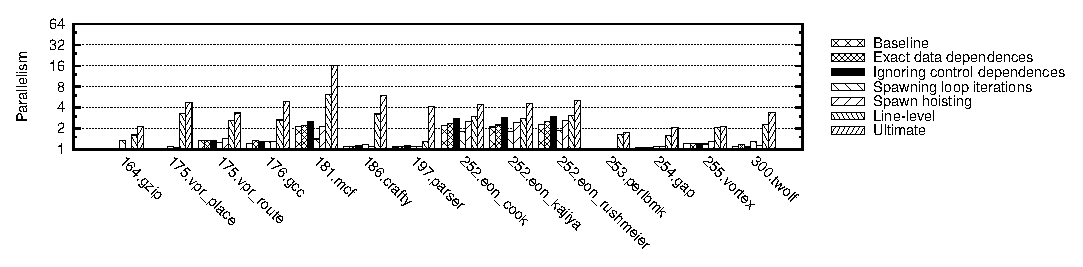
\includegraphics[width=4in]{spec}
% }
% \subfloat[SPEC CPU 2000 floating point benchmarks]{
%   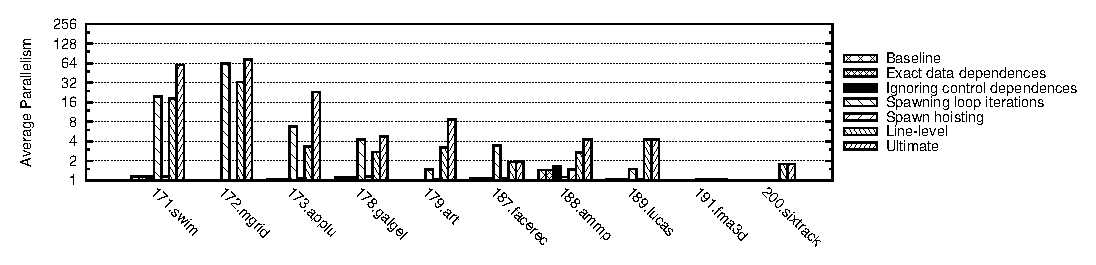
\includegraphics[width=4in]{specfp}
% }
% \subfloat[MiBench]{
%   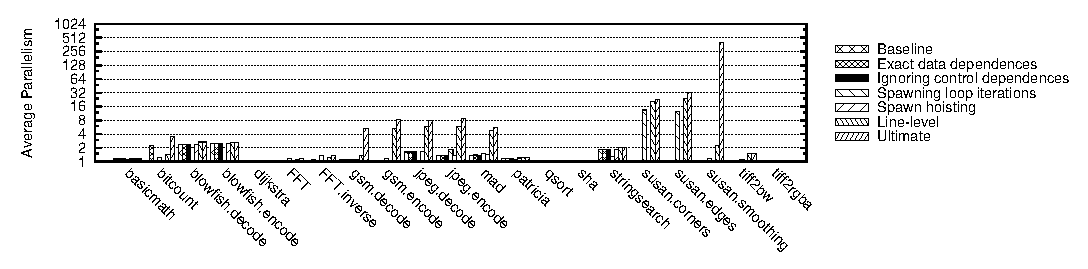
\includegraphics[width=4in]{mb}
% }
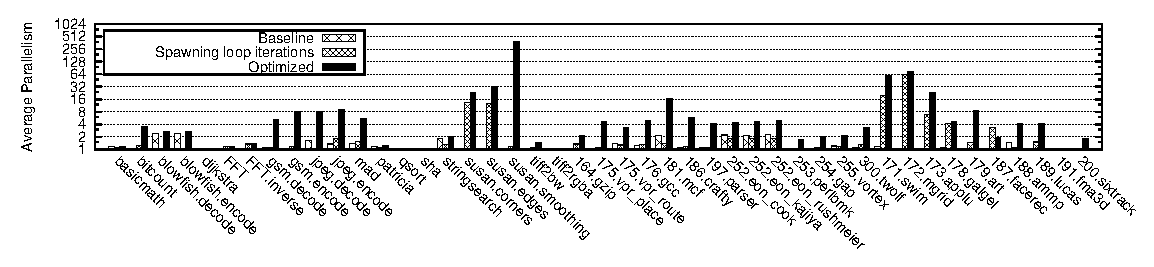
\includegraphics[width=5in]{benches}
\caption{Parallelism of benchmark programs}
\label{benchmarks}
\end{figure*}

We also ran the same analysis using Embla~2 on some of the benchmark programs in the SPEC CPU 2000~\cite{henning00spec} (with the MinneSPEC reduced data input set~\cite{KleinOsowski02minnespec}) and MiBench~\cite{guthaus01mibench} suites, the results of which are displayed in Figure~\ref{benchmarks}.
As before, the baseline model uses aggregated data dependences, and considers only function-call-level parallelism without loop parallelization or spawn hoisting.
The second model includes loop-level parallelism, while the third, \textsf{Optimized} model considers line-level parallelism and exact data dependences, hoisting spawns and ignoring control dependences.
In general, we see that few benchmarks exhibit the level of parallelism seen in the Cilk examples.
In fact, none of these benchmarks exhibit parallelism of over 3 under the baseline model,
suggesting that spawning existing function calls alone is insufficient to effectively parallelize them.

There are, however, some benchmarks with a significant amount of loop-level parallelism.
Some of them are the \textsf{susan} benchmarks from MiBench, which perform image smoothing, corner detection and edge detection on an image, and are data-parallel---the same computation is performed on each pixel in the image and the results for each pixel are independent of each other.
This is reflected in our results, which show that using the small inputs, both \textsf{susan.corners} and \textsf{susan.edges} have potential parallelism of over 12 when loop iterations are spawned.
This is not the case for \textsf{susan.smoothing}, however, as we will explain later.
Note that for some programs, e.g.\ \textsf{252.eon}, spawning loop iterations actually results in a lower level of parallelism than the baseline.
This is because the baseline allows for partial overlap between loop iterations (a.k.a.\ software pipelining) whereas spawning loop iterations is an all or nothing proposition; the iterations are either completely independent or completely serial.

\subsection{Increasing inherent parallelism by critical path analysis} \label{sresults:increasing}

Even though Embla~2 finds lots of inherent task-level parallelism in example programs from the Cilk test suite, little is found in most general-purpose programs, meaning they cannot be transformed into highly concurrent programs simply by spawning existing function calls and loops.
However, here Embla~2 can output the critical path of each function call, allowing us to examine the bottlenecks that prevent greater parallelism from being realized.
This critical path can then be collapsed into a graph with one node per line,
as shown in Figure~\ref{sha-critpath}.
We now demonstrate this in some of the simpler examples and suggest refactorings or algorithmic changes that would increase inherent parallelism.

\begin{figure*}[t]
 \centering
 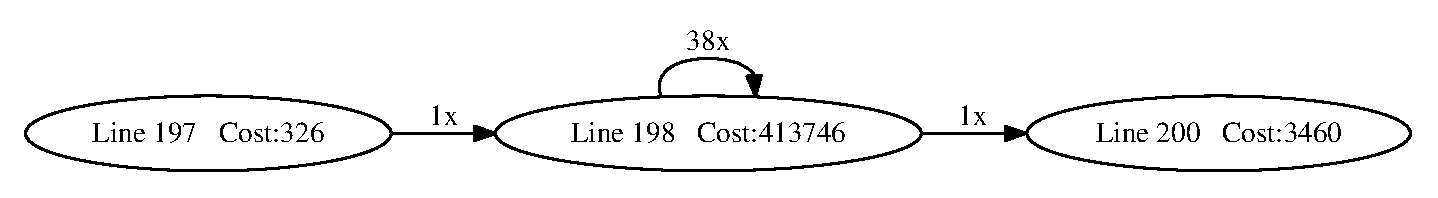
\includegraphics[width=4in]{sha_driver-c-24}
 \caption{Critical path of {\tt sha\_stream} function in \textsf{sha}}
 \label{sha-critpath}
\end{figure*}

\paragraph{\textsf{susan.smoothing}}

As mentioned, \textsf{susan.smoothing} is a data-parallel image smoothing application.
Unlike \textsf{susan.corners} and \textsf{susan.edges}, little inherent parallelism is found here (1.19 under the \textsf{Spawning loop iterations} model).
By examining the critical path, we found the main bottleneck dependence to be between instantiations of a certain loop within function \texttt{susan\_smoothing}.
Further examination of the loop reveals that the dependence is due to a variable that is incremented exactly once per iteration, and is therefore an induction variable.
However, as the increment is in the loop body rather than the loop header, each execution of the loop body is dependent on the last, and as a result iterations of the loops are serialized.
A simple solution is to move the increment operation to the loop header (manual code motion), which causes inherent parallelism to be vastly increased to around 1,090.

\paragraph{\textsf{sha}}

The Secure Hash Algorithm program computes a 160-bit hash value from the contents of an input file.
Under the \textsf{Line-level parallelism} variant model, Embla~2 reports a parallelism of 1.36.
Most of the critical path can be attributed to dependences between calls to
\texttt{sha\_update} (line 198 in Figure~\ref{sha-critpath}).
This function takes the existing hash value (the \emph{digest}) and derives a new hash value which replaces it.
Consequently, each call to this function must depend on the last as it requires the digest computed by the last call.
This suggests that in order to increase the amount of inherent parallelism, the underlying algorithm must be modified, e.g.\ by dividing the file into blocks and computing independent digests for each block, which are then combined into one final digest.

\paragraph{Other examples}

Applying the same analysis to other examples, we find that input/output forms a large part of several benchmarks.
In \textsf{dijkstra}, for example, a tenth of the program's sequential execution time is taken up by calls to \texttt{scanf}.
In \textsf{FFT} (MiBench), printing the results takes up around 80\% of processing time.
As input/output is unparallelizable without significant re-implementation, Amdahl's law would mean that the maximum speed-up, even if we were able to parallelize the rest of the program perfectly, would still be low.
This suggests that for some of the benchmarks examined, a parallel implementation of input/output would be very useful.










































%\section{Results} \label{sresults}
%
%\subsection{Parallelism in Cilk programs} \label{sresults:cilk}
%
%\begin{table}
%\small
%\begin{tabular}{ | l | l | l | }
%\hline
%Program & Description & Parameters \\
%\hline
%\textsf{cholesky} & Matrix decomposition & \texttt{size=256}, \texttt{nonzeros=1000} \\
%\textsf{cilksort} & Merge sort & \texttt{size=100000} \\
%\textsf{fft} & Fourier transform & \texttt{size=512*512} \\
%\textsf{fib} & Na\"ive Fibonacci calculation & \texttt{n=30} \\
%\textsf{heat} & Differential equation solver & \texttt{nx=ny=512}, \texttt{nt=1} \\ 
%\textsf{lu} & Matrix decomposition & \texttt{n=256} \\
%\textsf{magic} & Magic squares search & \texttt{n=4} \\
%\textsf{matmul} & Matrix multiplication & \texttt{n=128} \\
%\textsf{plu} & Matrix decomposition & \texttt{n=128} \\
%\textsf{strassen} & Matrix multiplication & \texttt{n=512} \\
%\hline
%\end{tabular}
%\caption{Description and parameters for Cilk 5.4.6 examples used}
%\label{cilk-ex}
%\end{table}
%
%We begin by presenting the results of analysing example Cilk programs packaged with the 5.4.6 release of Cilk, as described in Table~\ref{cilk-ex}\footnote{We have omitted programs that use the \texttt{inlet}, \texttt{abort} and \texttt{SYNCHED} keywords, as their translation into ordinary C is not straightforward.}.
%As examples packaged with a parallel programming environment, these are programs known to have lots of task-level parallelism.
%We ran the original programs in Cilk a number of times to obtain a figure for average parallelism as calculated by Cilk's timing infrastructure.
%We then translated these programs into semantically equivalent programs in ordinary C simply by stripping the Cilk keywords\footnote{Namely, \texttt{cilk}, \texttt{spawn} and \texttt{sync}.}.
%These \emph{serial elisions} of the original programs are then analysed with our extension of Embla under a number of different models.
%
%\begin{figure}
% \centering
% 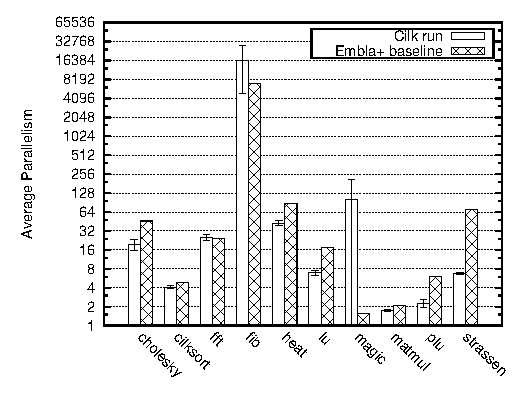
\includegraphics[width=2.9in]{cilk-run}
% \caption{Parallelism of Cilk programs as calculated by Cilk and Embla}
% \label{cilk-run}
%\end{figure}
%
%Figure~\ref{cilk-run} compares the parallelism found by Cilk (averaged over 60 runs) to that found by our extension of Embla on their serial elisions.
%Our baseline model for this comparison uses aggregated data dependences and control dependences, and considers only function-call-level parallelism without loop parallelization or spawn hoisting---the closest model we have to Cilk's.
%The graph shows that our tool is able to find all of the task-level parallelism in most of the original Cilk programs.
%The only exceptions are \textsf{fib} and \textsf{magic}, the Cilk parallelism for which appears to vary greatly.
%The reason our tool does not find much parallelism in \textsf{magic} compared to the Cilk run is because the Cilk program uses an associative reduction variable in a loop which sums over the results of each iteration, in the form \texttt{for (...) count += spawn(...);}.
%Our tool does not currently recognize associative reduction variables, and therefore cannot discover such parallelism.
%
%\begin{figure}[t]
%  \begin{center}
%  \scriptsize
%  \input{cilksort.depgraph}
%  \end{center}
%  \caption{An extract from \textsf{cilksort} and its corresponding relevant dependences}
%  \label{cilksort-depgraph}
%\end{figure}
%
%Using aggregated dependences discovered by our tool it is easy to re-insert Cilk keywords into the program to materialize the parallelism discovered.
%As an example, Figure~\ref{cilksort-depgraph} shows the aggregated dependences that our tool found for an extract from the \textsf{cilksort} program.
%Observe that simply by inserting \texttt{spawn}s in front of function calls, and \texttt{sync}s before the first line that depends on previously spawned tasks, we arrive at the original program.
%
%\begin{figure}
%  \begin{center}
%  \scriptsize
%  \begin{SubFloat}{\label{cilk-sync:without}Original program, showing dependences and best possible parallelization with universal \texttt{sync}s}
%    \begin{minipage}{3in}
%      \input{lu.depgraph}
%    \end{minipage}%
%  \end{SubFloat}%
%\\
%  \begin{SubFloat}{\label{cilk-sync:with}Best possible parallelization if individual \texttt{sync}s were allowed}
%    \begin{minipage}{3in}
%      \begin{verbatim}
%future1 = spawn schur(M00, V00, W00, hnb);
%future2 = spawn schur(M01, V00, W01, hnb);
%future3 = spawn schur(M10, V10, W00, hnb);
%future4 = spawn schur(M11, V10, W01, hnb);
%
%sync future1;
%spawn schur(M00, V01, W10, hnb);
%sync future2;
%spawn schur(M01, V01, W11, hnb);
%sync future3;
%spawn schur(M10, V11, W10, hnb);
%sync future4;
%spawn schur(M11, V11, W11, hnb);
%      \end{verbatim}
%    \end{minipage}%
%  \end{SubFloat}%
%  \end{center}
%  \caption{An example of the greater parallelism caused by individual \texttt{sync}s in an extract from \textsf{lu}.}
%  \label{cilk-sync}
%\end{figure}
%
%
%In fact, for a few examples our tool can discover more parallelism than explicitly specified in the original Cilk program.
%We found functions called sequentially in \textsf{cholesky}, \textsf{heat} and \textsf{strassen} that could have been spawned.
%In addition, we also found C library function calls in \textsf{heat}, \textsf{lu} and \textsf{plu} that cannot be spawned directly in Cilk (as library functions are not defined as spawnable) but can be spawned with the addition of simple wrappers.
%The greater parallelism found in \textsf{cholesky}, \textsf{lu} and \textsf{plu} can also be partly attributed to a restriction in Cilk that \texttt{sync}s must join on all tasks spawned rather than any individual task.
%If tasks could be synchronized on individually, as illustrated in Figure~\ref{cilk-sync}, then greater parallelism may be found.
%
%We now look more closely at the various models used to examine whether they affect potential parallelism in these programs.
%
%\subsubsection{Data dependences}
%
%\begin{figure}
% \centering
% 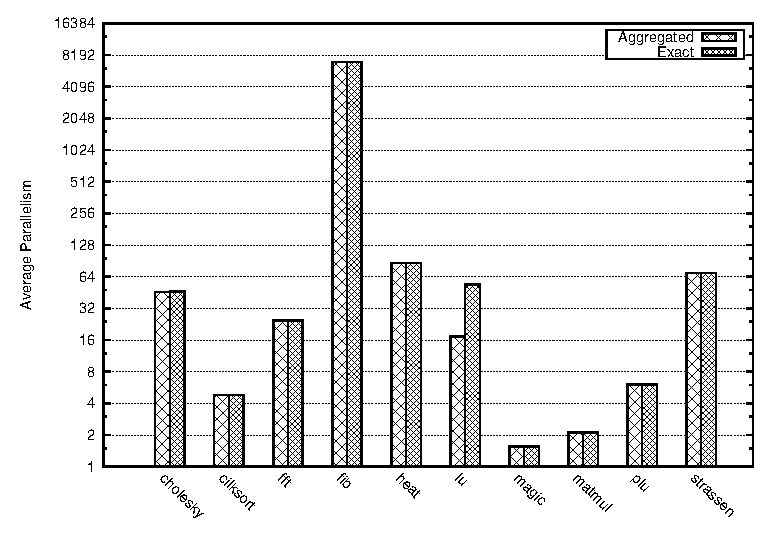
\includegraphics[width=2.9in]{cilk-data}
% \caption{Parallelism of Cilk programs with aggregated and exact data dependences}
% \label{cilk-data}
%\end{figure}
%
%Figure~\ref{cilk-data} shows the potential parallelism of the serial elisions of our Cilk examples with aggregated and exact data dependences.
%In all programs but \textsf{lu} we see that the difference between the two models is negligible.
%This suggests that for most programs most of the potential parallelism is achievable by adding parallel constructs at the source level---runtime techniques such as thread-level speculation would give few performance benefits.
%
%\subsubsection{Control dependences}
%
%%\begin{figure}
%% \centering
%% 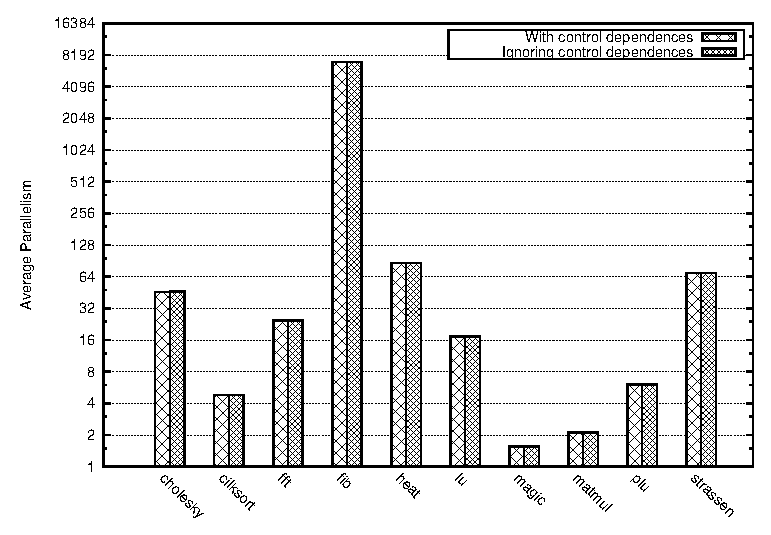
\includegraphics[width=2.9in]{cilk-ctl}
%% \caption{Parallelism of Cilk programs with and without control dependences}
%% \label{cilk-ctl}
%%\end{figure}
%
%%The effects of control speculation are shown in Figure~\ref{cilk-ctl}, which compares the parallelism when control dependences are considered to that when they are ignored.
%In all of the programs examined the parallelism is virtually unchanged, when control dependences are ignored, compared to the baseline figures in Figure~\ref{cilk-run}.
%This means that for these programs control speculation does not have any effect on available parallelism.
%One possible reason for this is that most of these programs are stream-processing-like, with few branches that depend on the data input.
%More irregular programs may see greater improvements with control speculation.
%
%\subsubsection{Granularity}
%
%\begin{figure}
% \centering
% 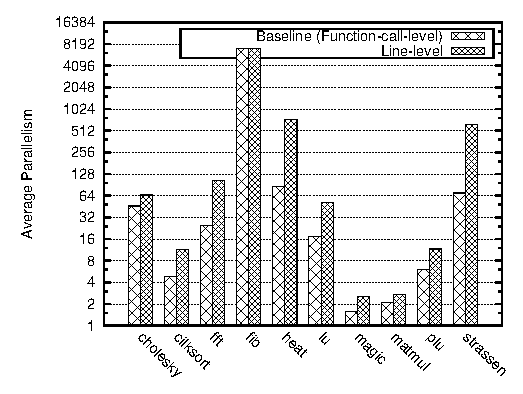
\includegraphics[width=2.9in]{cilk-gran}
% \caption{Parallelism of Cilk programs with different levels of granularity}
% \label{cilk-gran}
%\end{figure}
%
%The amount of line-level parallelism in these programs is compared to the amount of task-level parallelism in Figure~\ref{cilk-gran}.
%We can see that for most of these programs the amount of line-level parallelism is around twice or more the amount of function-call-level parallelism.
%Most of this difference is due to simple statements that perform arithmetic operations inside a function call or loop that can run in parallel.
%Each of these operations takes a small number of cycles, which means that it is not viable for each of these to be spawned.
%Nevertheless, operations may be grouped and extracted into tasks that are sufficiently large to see performance gains.
%We also note that some of this parallelism may well be realized already in existing superscalar or VLIW processors.
%
%\subsubsection{Loops}
%
%\begin{figure}
% \centering
% 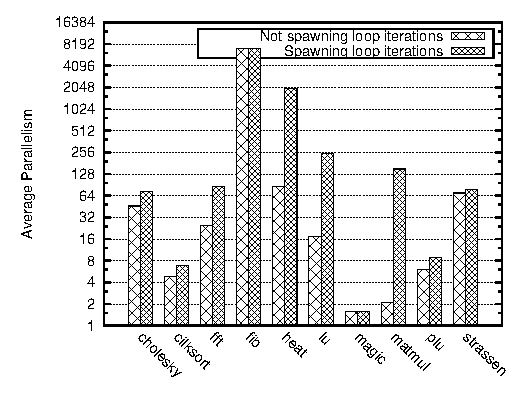
\includegraphics[width=2.9in]{cilk-loop}
% \caption{Parallelism of Cilk programs with and without spawning loop iterations}
% \label{cilk-loop}
%\end{figure}
%
%Looking at Figure~\ref{cilk-loop}, which compares the potential parallelism of Cilk programs with and without spawning loop iterations, we can see that the use of parallel for-loops benefit most of the programs considered here.
%This is most remarkable in \textsf{matmul}, where there is a 64-fold gain in parallelism when for-loops are parallelized.
%We deduce from this that the use of parallel for-loops is an excellent way to express task-level parallelism, in addition to function calls.
%Indeed, this justifies the inclusion of parallel for-loops in Cilk++, the commercialized version of Cilk.
%Our extension of Embla not only finds the amount of loop-level parallelism in a program, but can be used to easily identify candidate loops for parallelization.
%This can simply be done by searching through the dependences output by our tool for dependences between iterations of the loop concerned.
%If there are no such dependences, then the loop can be parallelized.
%
%\subsubsection{Spawn hoisting}
%
%%\begin{figure}
%% \centering
%% 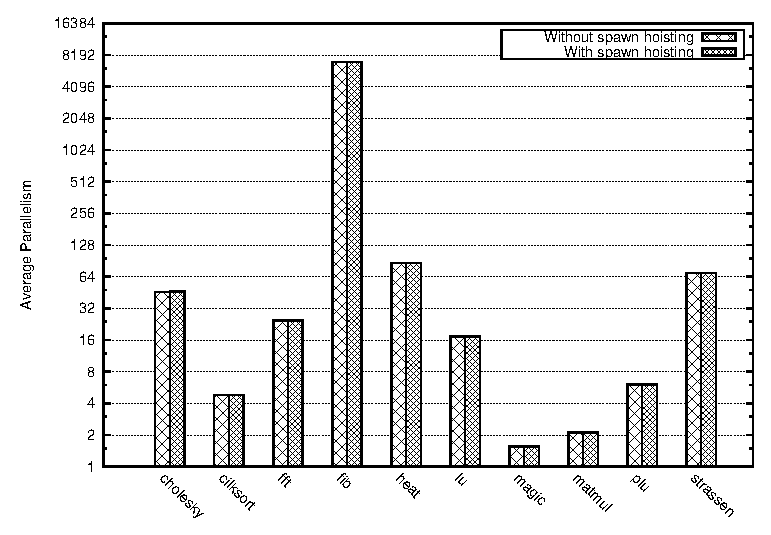
\includegraphics[width=2.9in]{cilk-hoist}
%% \caption{Parallelism of Cilk programs with and without spawn hoisting}
%% \label{cilk-hoist}
%%\end{figure}
%
%%Figure~\ref{cilk-hoist} shows little effect of spawn hoisting on the amount of potential parallelism in the Cilk examples.
%With our programs, we find that spawn hoisting has a negligible effect on the amount of potential parallelism in the Cilk examples, as parallelism measurements using spawn hoisting is almost the same as those for the baseline in Figure~\ref{cilk-run}.
%This suggests that most function calls are already spawned at the earliest possible point in the program, and there is little further hoisting possible.
%
%\subsection{Parallelism in various benchmarks}
%
%\begin{figure*}
% \centering
% \subfloat[SPEC CPU 2000 integer benchmarks]{
%   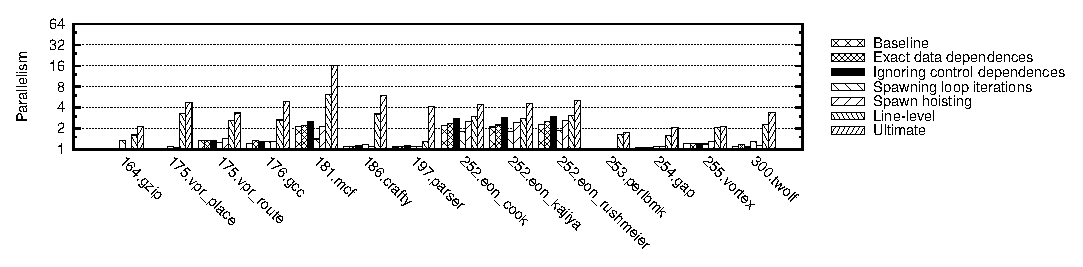
\includegraphics[width=6in]{spec}
% }
% \subfloat[SPEC CPU 2000 floating point benchmarks]{
%   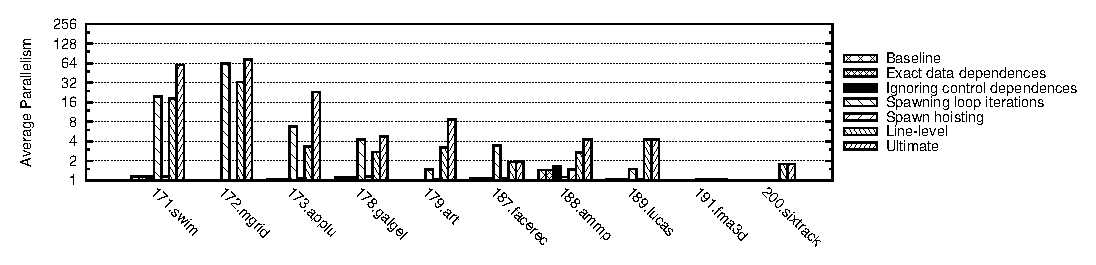
\includegraphics[width=6in]{specfp}
% }
% \subfloat[MiBench]{
%   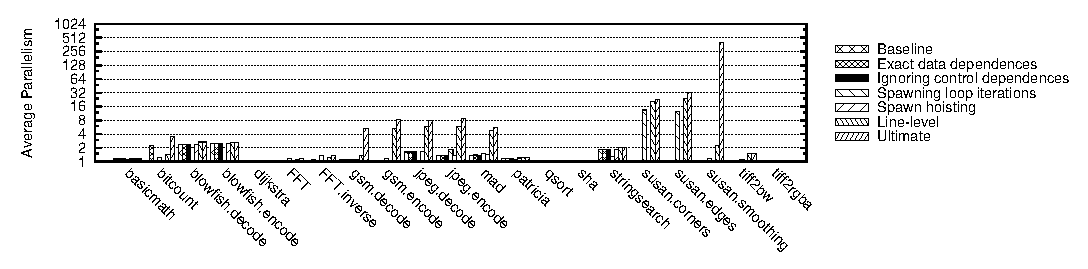
\includegraphics[width=6in]{mb}
% }
%
%\caption{Parallelism of three benchmark suites under various models}
%\label{benchmarks}
%\end{figure*}
%
%We also ran the same analysis using our tool on some of the benchmark programs in the SPEC CPU 2000 (with the MinneSPEC reduced data input set \cite{KleinOsowski02minnespec}) and MiBench suites, the results of which are displayed in Figure~\ref{benchmarks}.
%As before, the baseline model uses aggregated data dependences and control dependences, and considers only function-call-level parallelism without loop parallelization or spawn hoisting.
%Each of the other models differs from the baseline by one parameter described in Section~\ref{smethod}, except for \textsf{Ultimate}, which considers line-level parallelism by using exact data dependences, ignoring control dependences and hoisting spawns.
%In general, we see that few benchmarks exhibit the level of parallelism seen in the Cilk examples.
%In fact, none of these benchmarks exhibit parallelism of over 3 under the baseline model.
%
%There are, however, some benchmarks with a significant amount of loop-level parallelism.
%One of them is the MiBench benchmark \textsf{susan}, a program that performs image smoothing, corner detection and edge detection on an image, and is data-parallel---the same computation is performed on each pixel in the image and the results for each pixel are independent of each other.
%This is reflected in our results, which show that both \textsf{susan.corners} and \textsf{susan.edges} have potential parallelism of over 12 when loop iterations are spawned.
%This is not the case for \textsf{susan.smoothing}, however, as we will explain later.
%
%We note also that for some programs, e.g.\ \textsf{252.eon}, spawning loop iterations actually results in a \emph{lower} level of parallelism.
%This is because that while spawning loop iterations allows us to exploit DOALL parallelism, where loop iterations are completely independent from each other and can be executed in parallel, it precludes DOACROSS parallelism or software pipelining, where there are cross-iteration dependences but loop iterations can still partially overlap.
%The balance between DOALL and DOACROSS loops would therefore determine whether parallelism rises or falls compared to the baseline.
%
%\subsection{Increasing inherent parallelism by Critical path analysis} \label{sresults:increasing}
%
%Our results suggest that while the example programs from Cilk have lots of inherent task-level parallelism, most general-purpose programs tend to have little and cannot be transformed into highly concurrent programs simply by spawning existing function calls and loops.
%Nevertheless, our extension of Embla can output the critical path of each function call, allowing us to examine the bottlenecks that prevent greater parallelism from being realized.
%Here we demonstrate the use of critical path information to locate bottlenecks in some of the simpler examples and suggest refactorings or algorithmic changes that would increase inherent parallelism.
%
%\subsubsection{\textsf{sha}}
%
%\begin{figure}
%  \begin{center}
%    \scriptsize
%    \begin{SubFloat}{\label{sha-bottleneck:critpath}Critical path for a call to the \texttt{sha\_stream} function, produced by our tool}
%      \begin{minipage}{3in}
%        \begin{verbatim}
%!sha_driver.c:24(sha.c)=16139892:
%200(3460), 198(26614), 198(423934), 198(423934),
%198(423934), 198(423934), 198(423934), 198(423934),
%198(423934), 198(423934), 198(423934), 198(423934),
%198(423934), 198(423934), 198(423934), 198(423934),
%198(423934), 198(423934), 198(423934), 198(423934),
%198(423934), 198(423934), 198(423934), 198(423934),
%198(423934), 198(423934), 198(423934), 198(423934),
%198(423934), 198(423934), 198(423934), 198(423934),
%198(423934), 198(423934), 198(423934), 198(423934),
%198(423934), 198(423934), 198(423934), 198(423934),
%197(326)
%        \end{verbatim}
%      \end{minipage}
%    \end{SubFloat}
%\\
%    \begin{SubFloat}{\label{sha-bottleneck:source}Source for \texttt{sha\_stream} function in \texttt{sha.c}}
%      \begin{minipage}{3in}
%        \begin{verbatim}
%191  void sha_stream(SHA_INFO *sha_info, FILE *fin)
%192  {
%193      int i;
%194      BYTE data[BLOCK_SIZE];
%195
%196      sha_init(sha_info);
%197      while ((i = fread(data, 1, BLOCK_SIZE, fin)) > 0) {
%198          sha_update(sha_info, data, i);
%199      }
%200      sha_final(sha_info);
%201  }
%        \end{verbatim}
%      \end{minipage}
%    \end{SubFloat}
%  \end{center}
%  \caption{Critical Path Analysis of SHA}
%  \label{sha-bottleneck}
%\end{figure}
%
%\textsf{Sha}, or Secure Hash Algorithm, is a program that computes a 160-bit hash value from the contents of an input file.
%Figure~\ref{sha-bottleneck} illustrates part of our analysis into the reason for the lack of inherent parallelism there.
%Under the `Line-level' model, our tool reports a critical path of length 16,150,120 instructions out of the total work of 21,968,394 instructions, resulting in a parallelism of 1.36.
%From Figure~\ref{sha-bottleneck:critpath}, we see that most of the critical path (16,139,892 instructions) can be attributed to a function call on line 24 in the file \texttt{sha\_driver.c}.
%We also see that the critical path consists mainly of dependences between instantiations of line 198 in \texttt{sha.c}, most of which have a cost of 423,934 instructions.
%These correspond to calls to \texttt{sha\_update} in the program source (Figure~\ref{sha-bottleneck:source}).
%
%Further examination of \texttt{sha\_update} reveals that the function takes the existing hash value (the \emph{digest}) and derives a new hash value which replaces it.
%Consequently, each call to this function must depend on the last as it requires the digest computed by the last call.
%This suggests that in order to increase the amount of inherent parallelism, the underlying algorithm must be modified, e.g.\ by dividing the file into blocks and computing independent digests for each block, which are then combined into one final digest.
%
%\subsubsection{\textsf{susan.smoothing}}
%
%\begin{figure}
%  \begin{center}
%    \scriptsize
%    \begin{SubFloat}{\label{susan-bottleneck:critpath}Critical path for a call to the \texttt{susan\_smoothing} function, produced by our tool}
%      \begin{minipage}{3in}
%        \begin{verbatim}
%!susan.c:2057(susan.c)=37137459:
%-9(390875), -9(390875), -9(390875), -9(390875),
%-9(390875), -9(390875), -9(390875), -9(390875),
%-9(390875), -9(390875), -9(390875), -9(390875),
%...
%-9(390875), -9(390875), -9(390875), -9(390875),
%-9(390875), -9(390875), -9(390875), -13(147),
%-13(147), -13(147), -13(147), -13(147), 
%...
%        \end{verbatim}
%      \end{minipage}
%    \end{SubFloat}
%\\
%    \begin{SubFloat}{\label{susan-bottleneck:source}Source for loop concerned function in \texttt{susan.c}}
%      \begin{minipage}{3in}
%        \begin{verbatim}
%738    for (i=mask_size;i<y_size-mask_size;i++) // loop 9
%739    {
%740      for (j=mask_size;j<x_size-mask_size;j++) // loop 10
%741      {
%742        area = 0;
%743        total = 0;
%744        dpt = dp;
%745        ip = in + ((i-mask_size)*x_size) + j - mask_size;
%746        centre = in[i*x_size+j];
%747        cp = bp + centre;
%748        for(y=-mask_size; y<=mask_size; y++) // loop 11
%749        {
%750          for(x=-mask_size; x<=mask_size; x++) // loop 12
%751          {
%752            brightness = *ip++;
%753            tmp = *dpt++ * *(cp-brightness);
%754            area += tmp;
%755            total += tmp * brightness;
%756          }
%757          ip += increment;
%758        }
%759        tmp = area-10000;
%760        if (tmp==0)
%761          *out++=median(in,i,j,x_size);
%762        else
%763          *out++=((total-(centre*10000))/tmp);
%764      }
%765    }
%        \end{verbatim}
%      \end{minipage}
%    \end{SubFloat}
%  \end{center}
%  \caption{Critical Path Analysis of \textsf{susan.smoothing}}
%  \label{susan-bottleneck}
%\end{figure}
%
%Not all the changes required are as drastic, however.
%As mentioned, \textsf{susan.smoothing} is a data-parallel image smoothing application.
%Unlike \textsf{susan.corners} and \textsf{susan.edges}, little inherent parallelism is found here even when loop iterations are spawned.
%Under the `Spawning loop iterations' model of parallelism, our tool has reported a critical path length of 37,168,389 instructions out of a total of 44,240,209 instructions, resulting in a parallelism of 1.19.
%Most of the critical path can be attributed to the function call \texttt{susan\_smoothing}, the critical path of which is shown in Figure~\ref{susan-bottleneck:critpath}.
%From the critical path we deduce that the main dependence is one between instantiations of Loop~9 (the minus sign denotes a loop number rather than line number), which is the outermost loop shown in Figure~\ref{susan-bottleneck:source}.
%
%Further examination of the loop reveals that the dependence is due to increments to variable \texttt{out} on lines 761 and 763.
%This variable is incremented exactly once per iteration of Loop~10, and is therefore an induction variable.
%However, as the increment is in the loop body rather than the loop header, each execution of the loop body is dependent on the last, and as a result iterations of the loops are serialized.
%Indeed, simply moving the increment of \texttt{out} to the loop header causes inherent parallelism to be vastly increased to around 1,090.
%
%\subsubsection{Other examples}
%
%Applying the same analysis to other examples, we find that input/output forms a large part of several benchmarks.
%In \textsf{dijkstra}, for example, a tenth of the program's sequential execution time is taken up by calls to \texttt{scanf}.
%In \textsf{FFT} (MiBench), printing the results takes up around 80\% of processing time.
%As input/output is unparallelizable without significant re-implementation, Amdahl's law would mean that the maximum speed-up, even if we were able to parallelize the rest of the program perfectly, would still be low.
%This suggests that for some of the benchmarks examined, a parallel implementation of input/output would be very useful.
%
%\subsection{Getting more parallelism from loops}
%
%\begin{figure}
%  \centering
%  \small
%  \begin{SubFloat}{\label{dnc:orig}Original program}
%    \begin{minipage}{3in}
%      \begin{verbatim}
%for (j = n = 0, seed = rand();
%     j < iterations;
%     j++, seed += 13) {
%  int r = pBitCntFunc[i](seed);
%  n += r;
%}
%      \end{verbatim}
%    \end{minipage}%
%  \end{SubFloat}%
%\\
%  \begin{SubFloat}{\label{dnc:trans}Transformed program}
%    \begin{minipage}{3in}
%      \begin{verbatim}
%int dc_bitcnts(int start, int n_itrs, int i) {
%  if (n_itrs <= 0) return 0;
%  if (n_itrs == 1) return pBitCntFunc[i](start);
%  else {
%    int x,y;
%    int half_itrs = n_itrs / 2;
%    x = dc_bitcnts(start, half_itrs, i);
%    y = dc_bitcnts(start+(half_itrs*13),
%          n_itrs - half_itrs, i);
%    return x+y;
%  }
%}
%
%n = dc_bitcnts(rand(), iterations, i);
%      \end{verbatim}
%    \end{minipage}%
%  \end{SubFloat}%
%  \caption{Transformation of a loop in the \textsf{bitcount} program using divide and conquer.}
%  \label{dnc}
%\end{figure}
%
%It is in fact possible to amplify the level of parallelism in parallel for-loops.
%Figure~\ref{dnc} shows a transformation applied to a (slightly adapted) loop from the \textsf{bitcount} benchmark.
%In the original program, calls to \texttt{pBitCntFunc[i]} are pure and can be run in parallel with each other.
%However, there is a dependence between increments of the induction variables, \texttt{j} and \texttt{seed}, and between additions to the accumulator \texttt{n}, producing two long chains of data dependences.
%Nevertheless, by recognising that \texttt{n} is a reduction variable we can transform the loop into recursive calls using a divide-and-conquer strategy.
%The lengths of the dependence chains on the induction and reduction variables become logarithmic on the number of iterations instead of linear, and consequently the critical path found by our tool is a tenth of that in the original program, despite the overheads of extra function calls.
%This shows that simple transformations can sometimes be sufficient to increase the amount of potential parallelism in certain programs.
%In fact, we note that Cilk++ indeed uses a divide-and-conquer strategy for its parallel for-loops, a decision which is justified by our example.
%
